%--------------PREAMBLE------------------------------------------------------

%This is your preamble where you decide which packages to load and which document class you want to use. This is also where you use all commands you want to define for the whole document. (The preamble is not printed).

%--------------DOCUMENT CLASS -----------------------------------------------
\documentclass[a4paper, 12pt]{article} %defines the document class and specifies paper size and font size

%--------------PACKAGES------------------------------------------------------

%\usepackage{fontspec} %works with XeLaTeX to make unicode input work and lets you choose fonts
%\setmainfont{Cambria} %sets the main font
%\setsansfont{Calibri} %sets the sans serif font
%\setmonofont{Courier New} %sets the mono-spaced font

\usepackage[affil-it]{authblk}
%\usepackage{polyglossia}
%\setdefaultlanguage{english}
%\setmainlanguage{english}
%\setotherlanguage{french, german}

\usepackage[british]{babel}

\usepackage{hyperref}

\usepackage{forest}
\useforestlibrary{linguistics}
\forestapplylibrarydefaults{linguistics}
\usepackage{soul}
\usepackage{graphicx}
\usepackage{tipa}

\usepackage{xcolor} %lets you use colours

\usepackage[citestyle=apa, backend=biber, maxbibnames=99]{biblatex}
\addbibresource{workshop.bib}

%----------TITLE-------------------------------------------------------------

\title{Workshop Handout} %defines the title
\author{Nina Markl$^1$ \& Brandon Papineau$^2$} %defines the authors
\date{%
    $^1$The University of Edinburgh\\%
    $^2$Stanford University\\[2.5ex]
16 April 2021} %defines the date - this can also be set to \today

\usepackage{gb4e} % gb4e needs to go last, right before "\begin{document}" - no knows why

\begin{document} %begins the document

\maketitle %prints your title
\tableofcontents %prints all sections, subsections etc.
\pagebreak %inserts a pagebreak


\begin{abstract} %This defines an abstract environment, which can automatically format your abstract for you
    This is an example paper all about using \LaTeX in linguistics. This is a workshop being run by Nina Markl (PhD student, University of Edinburgh) and Brandon Papineau (PhD student, Stanford University) at the Undergraduate Linguistics Association of Britain conference, 2021. We are grateful to the local hosts for inviting us to participate in this event, and we hope you learn lots.
\end{abstract}

\section{Introduction} %begins a section

This document contains some examples for a simple article.

\subsection{Here's a subsection}

\subsubsection{And a subsubsection}

\paragraph{And a paragraph}

\section{Literature Review}

To cite important scholars in your field (or up-and-coming ones like us), you set up a .bib file which contains all relevant information for each bibliography entry. Every entry has a unique key, which you use to create in-text citations, using \textcite[15]{papineauhooked} or \parencite[27]{burchell-etal-2020-querent} if you want the citation to go in brackets.

You can also easily add footnotes\footnote{like this}.


\section{Adding Figures \& Examples}

\subsection{Floats}

One of the advantages of \LaTeX over, say, MS Word, is the way it handles floats (tables and figures). It's very easy to attach a caption and a label to a figure. By default \LaTeX will place floats where there's enough space, but you can specify where a figure is placed.

\subsubsection{Tables}

\LaTeX automatically places floats wherever there is space - if there is not enough space on the current page it will push it to a new page. The automatic placement can be overridden by specific placement commands:

\begin{table}[h!]
	\centering
	\begin{tabular}{|l l|} \hline
	\textbf{Spec} & \textbf{Placement permission}\\ \hline
	h & right here \\ \hline
	t & at the top of a page \\\hline
	b & at the bottom of a page \\\hline
	p & on a page with other floats \\\hline
	! & ignore internal specifications such as maximal number of floats on a page \\ \hline
	\end{tabular}
\caption{Placement specifications for floats.}
\end{table}

\noindent You can also force \LaTeX to print all floats you have defined so far via the command $\backslash$\texttt{clearpage}.

\noindent The actual rows and columns of a table are defined in the \texttt{tabular} environment. If you put this \texttt{tabular} into a \texttt{table} environment (a floating environment), you will be able to refer back to it, add captions, etc. To create prettier tables, use the package \texttt{booktabs} (with slightly different syntax).

\begin{verbatim}
\begin{table}[h!]
\centering
\begin{tabular}[c]{|l l|} \hline
command & output  \\ \hline
l & left-aligned  \\ \hline
r & right-aligned  \\ \hline
c & centred \\ \hline
\end{tabular}
\caption{This is a tabular showing you how to tabular (table spec).}
\label{tabular}
\end{table}
\end{verbatim}
\begin{table}[h!]
	\centering
\begin{tabular}[c]{|l l|} \hline
	command & output  \\ \hline
	l & left-aligned  \\ \hline
	r & right-aligned  \\ \hline
	c & centred \\ \hline
\end{tabular}
\caption{This is a tabular showing you how to tabular (table spec).}
\label{tabular}
\end{table}
\noindent You can also have multiple columns under the same header (and the caption can also be above your tabular):


\begin{verbatim}
\begin{table}[ht!]
\centering
\caption{This is a complicated table describing complicated things.}
\begin{tabular}{|l l|} \hline
\multicolumn{2}{|c|}{\textbf{Complicated Table}} \\ \hline
Column 1 & Column 2 \\ \hline
Entry 1 & Entry 2 \\ \hline
\end{tabular}
\end{table}
\end{verbatim}

\begin{table}[ht!]
	\centering
	\caption{This is a complicated table describing complicated things.}
\begin{tabular}{|l l|} \hline
\multicolumn{2}{|c|}{\textbf{Complicated Table}} \\ \hline
Column 1 & Column 2 \\ \hline
Entry 1 & Entry 1\\ \hline
\end{tabular}
\end{table}



\subsubsection{Figures}

\paragraph{Inserting images into figures: graphicx and TikZ}
Images are also inserted into floating bodies in \LaTeX{}. One very useful package in this context is \texttt{graphicx}. Usually images are inserted into \texttt{figures}. To insert a graphic use the command $\backslash$\texttt{includegraphics[width OR height]\{filename\}}. Note that any labels you want to attach to the figure must immediately follow the caption. Make sure that the files are in the same folder as your \TeX{} file (or else provide the full path).

\begin{figure}
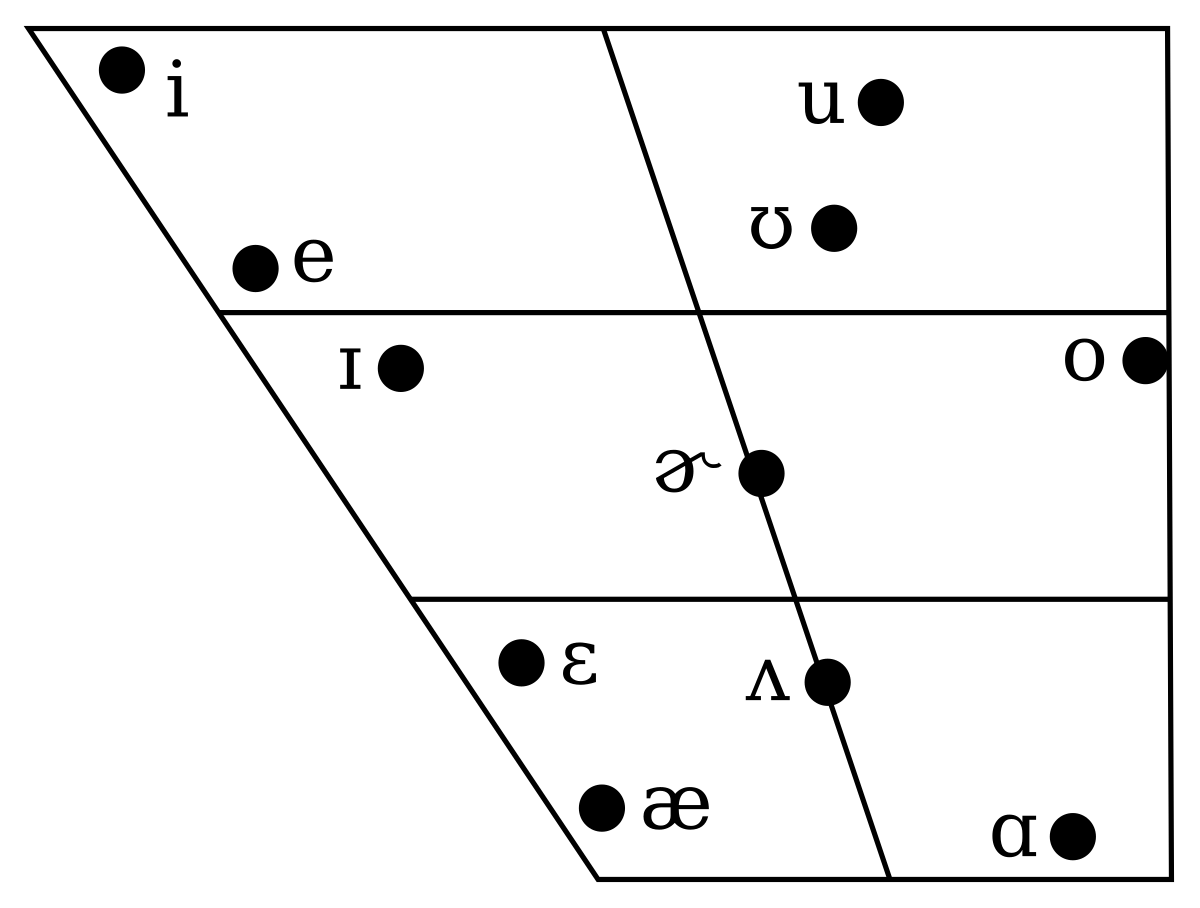
\includegraphics{vowelchart.png}
\caption{A caption for your image}\label{image}
\end{figure}

\begin{verbatim}

\begin{figure}
\includegraphics[width=\textwidth]{vowel_chart.png}
\caption{A caption for your image}\label{image}
\end{figure}
\end{verbatim}


\subsection{Examples}
Also critical to linguistics is the incorporation of examples! The most common implementation of these is gb4e, a package that is designed for exactly this. To implement an example, you use the exe environment and the ex command, like:

\begin{exe}
\ex This is a grammatically well-formed sentence.
\end{exe}

You'll frequently want to add grammaticality judgements or the like to sentences, which you can do with a simple change to the command, as in:

\begin{exe}
\ex[*] {This sentence is grammatically well-formed not}
\end{exe}

Just remember to bracket your sentence if you're doing this! The nice thing about gb4e is that it also automatically updates the enumerations of your examples, so you don't need to keep track of what you previously labelled each example! \par
You can also use gb4e to give nested sub-examples! This can be really helpful when comparing, for example, related but distinct grammaticality judgements or examples from different languages. You just need to embed the xlist environment. For example:

\begin{exe}
\ex The Germanic languages
    \begin{xlist}
        \ex English is a West Germanic language.
        \ex Deutsch ist auch eine Westgermanische Sprache.
    \end{xlist}
\end{exe}

Finally, gb4e's exe environment allows you to embed all sorts of other things inside of it, like syntax trees or Optimality Theory tableaux. Just to exemplify this (if you're curious about the syntax of the forest environment, you can check out the handbook we developed for this workshop).

\begin{exe}
    \ex
    \begin{forest}
        [T [N [linguistics]]
        [T [T [\textsc{pres}]]
        [V [N [\st{linguistics}]]
        [V [V [is]]
        [ADJ [fun]]]]]]
    \end{forest}
\end{exe}

Finally, if you want to get into meta-\LaTeX-linguistics, you can highlight your example codes using the verbatim environment:

\begin{exe}
\ex Here is the above syntax tree, as a verbatim thing!

\begin{verbatim}
    \begin{exe}
    \ex
    \begin{forest}
        [T [N [linguistics]]
        [T [T [\textsc{pres}]]
        [V [N [\st{linguistics}]]
        [V [V [is]]
        [ADJ [fun]]]]]]
    \end{forest}
\end{exe}
\end{verbatim}

\end{exe}

\newpage
\printbibliography % to print the bibliography

\end{document}
